%%%%%%%%%%%%%%%%%%%%%%%%%%%%%%%%%%%%%%%%%%%%%%%%%%%%%%%%%%%
% --------------------------------------------------------
%  ____  _           
% |  _ \| |__   ___  
% | |_) | '_ \ / _ \ 
% |  _ <| | | | (_) |
% |_| \_\_| |_|\___/ 
%
% LaTeX2e Template
% Version 3.0.1 (15/04/2026)
%
% Author: 
% Guillermo Jimenez (memo.notess1@gmail.com)
% 
% Contributor:
% Eduardo Gracidas (eduardo.gracidas29@gmail.com)
%
% License:
% Creative Commons CC BY 4.0
% --------------------------------------------------------
%%%%%%%%%%%%%%%%%%%%%%%%%%%%%%%%%%%%%%%%%%%%%%%%%%%%%%%%%%%
% --------------------------------------------------------
% Find the latest version on GitHub:
% https://github.com/MemoJimenez/Rho-class
% --------------------------------------------------------
%%%%%%%%%%%%%%%%%%%%%%%%%%%%%%%%%%%%%%%%%%%%%%%%%%%%%%%%%%%

\documentclass[9pt,a4paper,twocolumn,twoside]{rho-class/rho}
\usepackage[english]{babel}

%% Spanish babel recomendation
% \usepackage[spanish,es-nodecimaldot,es-noindentfirst]{babel}

%----------------------------------------------------------
% Title
%----------------------------------------------------------

\doctype{Articol de cercetare}
\title{O analiză experimentală a algoritmilor de sortare uzuali. Când Sleep Sort câștigă.}

%----------------------------------------------------------
% Authors, Affiliations and dates
%----------------------------------------------------------

\author[{\textasteriskcentered},a,1]{Cristian Meriacri}


%----------------------------------------------------------

\affil[a]{Universitatea de Vest din Timișoara, Facultatea de Informatică, Str. Pârvan 4, Timișoara 300223, Romania - cristian.meriacri00@e-uvt.ro}


%----------------------------------------------------------

\dates{Acest articol a fost redactat în perioada Februarie-Mai 2026.}

%----------------------------------------------------------
% Corresponding author-, Document- information
%----------------------------------------------------------

%\corres{\textsuperscript{\textasteriskcentered}Corresponding author: \href{mailto:author.one@institute.org}{author.one@institute.org} (A. One).}
%\corres{\textsuperscript{\textdagger}These authors contributed equally to this work.}

%----------------------------------------------------------


%----------------------------------------------------------

%\journalname{LATEX}
%\journal{Rho-class (v.3) 2026}
%\theday{\today}
%\vol{X}
%\no{X}

%----------------------------------------------------------
% Abstract and Keywords
%----------------------------------------------------------

\begin{abstract}
    Această lucrare prezintă o analiză experimentală a performanței algoritmilor de sortare, comparând soluții clasice precum Bubble Sort, Insertion Sort, Quick Sort,Merge Sort și implementarea de referință din biblioteca standard C++, std::sort.
    Un element central și neconvențional al studiului este includerea algoritmului Sleep Sort, testat pentru a identifica limitele practice ale eficienței bazate pe multi-threading. 
    \\\\Metodologia a presupus implementarea în C++ folosind compilatorul GCC și testarea pe diverse seturi de date, cu dimensiuni cuprinse între $10$ și $2.000.000$ de elemente și cinci distribuții de valori diferite.
    Principalul parametru monitorizat a fost timpul de execuție, măsurat în timpul real de pe ceasul de perete folosind librăria standard inclusă chrono, pentru a evalua scalabilitatea și performanța fiecărui algoritm.
    \\\\Rezultatele obținute au evidențiat diferențe semnificative în performanță, cu algoritmi precum Quick Sort și Merge Sort demonstrând o eficiență superioară în comparație cu soluțiile mai simple.
    Totuși,deși majoritatea rezultatelor au fost pe măsura așteptărilor,bazat pe ce știm despre algoritmii de sortare, Sleep Sort a prezentat un comportament neașteptat, depășind performanța algoritmului std::sort din librăria C++ în anumite condiții.
    \\\\Lucrarea demonstrează astfel că eficiența unui algoritm este strâns legată de natura distribuției datelor și de dimensiunea acestora, evidențiind importanța alegerii algoritmului potrivit pentru fiecare situație specifică.
\end{abstract}

%----------------------------------------------------------

\keywords{Algoritmi, Sortare, Bubble Sort, Insertion Sort, Quick Sort, Merge Sort, Sleep Sort, std::sort, C++, Performanță, multi-threading, chrono}

%----------------------------------------------------------

\begin{document}
    \maketitle
    \thispagestyle{firststyle}

%----------------------------------------------------------
\tableofcontents
\newpage
\section{Introducere}

\rhostart{P}erformanța unui program depinde adesea mai mult de alegerea 
algoritmului decât de orice altă optimizare. În contextul sortării, una 
dintre operațiile cele mai frecvente în software, această alegere poate 
face diferența pe date reale, care rareori sunt perfect distribuite.


Această lucrare prezintă o analiză experimentală a șase algoritmi de 
sortare pe distribuții diverse, cu accent pe comportamentul lor în scenarii 
nefavorabile. Un element distinctiv este includerea Sleep Sort, un algoritm 
neconvențional bazat pe concurență, pentru a investiga dacă poate fi 
competitiv în condiții specifice.


Lucrarea este organizată astfel: Secțiunea~\ref{sec:algoritmi} descrie 
algoritmii, Secțiunea~\ref{sec:metodologie} prezintă configurația 
experimentală, Secțiunea~\ref{sec:rezultate} analizează rezultatele, 
iar Secțiunea~\ref{sec:concluzii} sintetizează concluziile.


\subsection{Declarație de originalitate}
Implementarea Sleep Sort propusă este propria mea contribuție: am observat 
că varianta clasică creează câte un thread per element, ineficient pe date 
cu duplicate, și am rezolvat asta grupând elementele identice printr-un 
\inlinecode{std::map} pe același fir de execuție.

\section{Date de Intrare}

    \subsection{Generalități}
    Această secțiune oferă o prezentare generală a datelor folosite în această lucrare, evidențiind principiile de funcționare și complexitatea lor teoretică.
    Algoritmii de sortare (mai puțin Sleep Sort) pot sorta orice tip de date, atâta timp cât există o relație de ordine definită între ele.
    
    Pe parcursul acestei lucrări,toate datele de intrare sunt de tip integer.

    \subsection{Tipuri de date}


    Fie $n \in \mathbb{N}$ dimensiunea șirului și $A = (a_1, a_2, \dots, a_n)$ 
un șir de numere întregi, $a_i \in \mathbb{Z}$. Algoritmii au fost testați 
pe cinci distribuții de date, alese pentru a acoperi scenarii reprezentative 
din practică.

\subsubsection{Aleatoriu}
$A$ este generat aleatoriu, unde fiecare $a_i \sim \mathcal{U}(1, 10^6)$, 
independent și uniform distribuit. Aceasta reprezintă cazul general, fără 
nicio structură prealabilă în date.

\subsubsection{Sortat Crescător}
$A$ este un șir sortat crescător, unde $a_i \leq a_{i+1}$ pentru orice 
$i = 1, \dots, n-1$. Reprezintă cel mai favorabil scenariu pentru algoritmii 
care exploatează ordinea existentă.

\subsubsection{Sortat Descrescător}
$A$ este un șir sortat descrescător, unde $a_i \geq a_{i+1}$ pentru orice 
$i = 1, \dots, n-1$. Reprezintă cazul defavorabil pentru majoritatea 
algoritmilor bazați pe comparații.

\subsubsection{Aproape Sortat}
$A$ este inițial sortat crescător, după care $\lfloor 0.01 \cdot n \rfloor$ 
perechi de elemente sunt interschimbate aleatoriu. Astfel, aproximativ $1\%$ 
din elemente sunt în afara poziției corecte, simulând date reale care au 
suferit modificări minore după o sortare anterioară.

\subsubsection{Plat}
$A$ este generat aleatoriu, unde $a_i \in \{v_1, v_2, v_3, v_4, v_5\}$, 
un set fix de exact 5 valori distincte. Această distribuție testează 
comportamentul algoritmilor în prezența unui număr foarte mare de duplicate.
    
    
    \section{Algoritmi de sortare}

    Această secțiune oferă o prezentare generală a algoritmilor de sortare analizați în această lucrare, evidențiind principiile de funcționare și complexitatea lor teoretică.

    \subsection{Bubble Sort}
    Bubble Sort este cel mai simplu algoritm de sortare, care funcționează prin compararea elementelor adiacente și interschimbarea lor dacă sunt în ordine greșită. Acest proces se repetă până când întregul șir este sortat.
    Deși este un algoritm foarte ineficient, Bubble Sort este adesea folosit în scop educațional pentru a ilustra conceptele de bază ale sortării.


    	\begin{rhoenv}[frametitle=Origine și popularitate]
            Originea acestui algoritm este incertă \cite{astrachan2003bubble}, fiind menționat sub diferite denumiri în literatura de specialitate ca "Sorting by Exchange", "Sinking Sort", "Jump Down", "Sink Down" sau "Exchange Sort".


Knuth l-a inclus în The Art of Computer Programming \cite{knuth1998sorting}, contribuind la consolidarea lui în literatura de specialitate, deși l-a criticat explicit.		\end{rhoenv}

    Complexitatea \cite{knuth1998sorting} a acestui algoritm este $O(n^2)$ în varianta de bază, fără optimizări, și $O(n)$ în cel mai favorabil caz (când șirul este deja sortat) dacă este folosită o implementare optimizată. În medie, complexitatea este tot $O(n^2)$, ceea ce îl face ineficient pentru șiruri mari.
   \newline Totodată,Bubble sort e mai încet decât alți algoritmi de sortare cu o complexitate $O(n^2)$ precum Insertion Sort sau Selection Sort (cu unele excepții evidențiate mai târziu), deoarece necesită mai multe interschimbări \cite{astrachan2003bubble} pentru a sorta șirul.
   \newline
   \newline Complexitatea de spațiu a acestui algoritm este $O(1)$, deoarece sortarea se face in-place (fără a aloca structuri de date auxiliare proporționale cu \textit{n}), fără a necesita spațiu suplimentar semnificativ.
\begin{code}
    \inputminted[style=friendly]{cpp}{cod_sursa/bubblesort.cpp}
    \caption{Implementarea Bubble Sort în C++.}
    \label{lst:bubblesort}
\end{code}


După cum se poate observa în codul sursă \ref{lst:bubblesort}, algoritmul parcurge șirul de la început până la sfârșit, comparând elementele adiacente și interschimbându-le dacă sunt în ordine greșită. Un flag numit swapped este folosit pentru a verifica dacă s-au făcut interschimbări în timpul unei treceri. Dacă nu s-a făcut nicio interschimbare, înseamnă că șirul este deja sortat și algoritmul se oprește, optimizând astfel cazul favorabil.
    

\subsection {Insertion Sort}

Insertion Sort funcționează prin construirea treptată a șirului sortat, 
inserând fiecare element în poziția corectă în raport cu cele deja sortate.
Prima mențiune documentată îi aparține lui John Mauchly în 1946, deși 
algoritmul era probabil folosit informal înainte \cite{knuth1998sorting}.

Algoritmul este eficient pentru șiruri mici sau aproape sortate, având o 
complexitate de $O(n)$ în cel mai favorabil caz și $O(n^2)$ în cazul mediu 
și defavorabil \cite{knuth1998sorting}. Complexitatea de spațiu este $O(1)$, 
deoarece sortarea se face in-place.

Knuth menționează că poziția de inserare poate fi găsită prin căutare binară 
\cite{knuth1998sorting}, reducând numărul de comparații la $O(\log n)$, fără 
a îmbunătăți însă complexitatea totală. O variantă mai agresivă, Gap Insertion 
Sort, folosește goluri între elemente pentru a reduce și mutările, obținând 
$O(n \log n)$ în majoritatea cazurilor \cite{bender2006insertionislogn}.

\begin{code}
    \inputminted[style=friendly]{cpp}{cod_sursa/insertionsort.cpp}
    \caption{Implementarea Insertion Sort în C++.}
    \label{lst:insertionsort}
\end{code}



Implementarea Insertion Sort prezentată în codul sursă \ref{lst:insertionsort} este o versiune clasică,fără optimizări ca căutarea binară pentru poziția de inserare menționată anterior.

\subsection{Merge Sort}

Merge Sort este un algoritm de sortare bazat pe paradigma divide et impera, care împarte șirul în subșiruri mai mici, le sortează recursiv și apoi le combină pentru a obține șirul sortat final. A fost inventat de John von Neumann în 1945 \cite{knuth1998sorting}.
Eficiența sa este de $O(n \log n)$ în toate cazurile,fără surprize sau cazuri excepționale, ceea ce îl face potrivit pentru șiruri mari. 
\newline Un dezavantaj al acestui algoritm este complexitatea de spațiu, care este $O(n)$, deoarece necesită un spațiu auxiliar pentru a stoca subșirurile în timpul procesului de combinare. Totodată,natura recursivă a algoritmului necesită un spațiu suplimentar pentru stiva de apeluri, ceea ce îl face ineficient pentru șiruri foarte mici sau pentru sisteme cu resurse limitate.

\begin{code}
    \inputminted[style=friendly]{cpp}{cod_sursa/mergesort.cpp}
    \caption{Implementarea Merge Sort în C++.}
    \label{lst:mergesort}
\end{code}

Implementarea prezentată în codul sursă \ref{lst:mergesort} folosește două funcții: \texttt{merge}, care combină două subșiruri sortate într-unul singur, și \texttt{mergeSort}, care realizează divizarea recursivă a șirului și apelează funcția de combinare.


\subsection{Quick Sort}

Quick Sort este un algoritm de sortare eficient, bazat pe paradigma divide et impera, care a fost inventat de Tony Hoare în 1959 și publicat în 1961 \cite{hoare1961quicksort}. Algoritmul funcționează prin alegerea unui element pivot din șir și împărțirea celorlalte elemente în două subșiruri: cele mai mici decât pivotul și cele mai mari decât pivotul. Acest proces se repetă recursiv pentru fiecare subșir până când întregul șir este sortat.

Quick Sort, în ciuda numelui său, nu garantează performanță 
superioară în toate cazurile \cite{hoare1961quicksort, knuth1998sorting}.
\footnote{Observație atribuită cursului de Algoritmi și Structuri 
de Date, Universitatea de Vest din Timișoara, de Prof. Dr. D. Zaharie.}
O problemă cunoscută a acestui algoritm este că performanța sa poate degrada la $O(n^2)$ în cazul în care pivotul ales este întotdeauna cel mai mic sau cel mai mare element, cum ar fi atunci când șirul este deja sortat sau sortat descrescător. Cu toate acestea, cu o alegere bună a pivotului (de exemplu, folosind metoda medianei), complexitatea medie și cea mai bună rămân $O(n \log n)$ \cite{knuth1998sorting}.
O misconcepție comună este că Quick Sort este întotdeauna mai rapid decât Merge Sort sau Bubble Sort, dar acest lucru nu este întotdeauna adevărat, deoarece Quick Sort are nevoie de mai mult overhead pentru gestionarea recursiei și poate fi ineficient pe șiruri mici sau aproape sortate, unde Insertion Sort sau Bubble Sort pot performa mai bine \cite{knuth1998sorting}. Aceeași problemă o suferă și Merge Sort.
Complexitatea de spațiu a Quick Sort este $O(\log n)$ în medie, datorită stivei de apeluri recursive, dar poate ajunge la $O(n)$ în cel mai defavorabil caz.

O optimizare separată, numită Algoritmul Flagului Olandez 
\cite{dijkstra1976discipline}, propusă de Dijkstra, modifică 
partiționarea pentru a gestiona eficient elementele duplicate — 
în loc de două zone (mai mic și mai mare decât pivotul), șirul 
este împărțit în trei: mai mic, egal și mai mare. Aceasta reduce 
semnificativ numărul de operații pe distribuții cu multe duplicate, 
cum ar fi distribuția plată din această lucrare.


\begin{code}
    \inputminted[style=friendly]{cpp}{cod_sursa/quicksort.cpp}
    \caption{Implementarea Quick Sort în C++.}
    \label{lst:quicksort}
\end{code}

Pentru a ilustra consecințele alegerii pivotului, implementarea prezentată în codul sursă \ref{lst:quicksort} folosește ultimul element ca pivot, ceea ce poate duce la performanță slabă pe șiruri deja sortate sau sortate descrescător. Pentru a evita acest lucru, se pot implementa strategii de alegere a pivotului, cum ar fi alegerea unui element aleatoriu sau folosirea medianei a trei elemente.

\subsection{std::sort}

std::sort este o funcție de sortare din biblioteca standard C++ care oferă o implementare optimizată, adaptată la dimensiunea și structura datelor. De obicei, std::sort utilizează o combinație de Quick Sort, Heap Sort și Insertion Sort, denumită Introsort \cite{musser1997introsort, cppreference_sort}.

Implementarea specifică poate varia între diferite compilatoare și platforme. În compilatorul GCC, std::sort folosește o variantă a Introsort care începe cu Quick Sort și comută la Heap Sort dacă adâncimea recursivă depășește un prag specificat, prevenind astfel degradarea la $O(n^2)$ pe șiruri sortate sau aproape sortate. Pentru subșiruri foarte mici, algoritmul folosește Insertion Sort, mai eficient în acest context.

Complexitatea std::sort este $O(n \log n)$ în toate cazurile \cite{musser1997introsort}, inclusiv cel defavorabil. Complexitatea de spațiu este $O(\log n)$, datorită stivei de recursivitate. Algoritmul nu este stabil — pentru stabilitate, biblioteca standard oferă \texttt{std::stable\_sort}.

Codul sursă al std::sort nu este unic, fiind adaptat diferitelor platforme și compilatoare. O implementare de referință a Introsort poate fi găsită în literatura de specialitate \cite{musser1997introsort}, iar implementarea din GCC este disponibilă în fișierul \texttt{bits/stl\_algo.h} \cite{gcc_stl_algo}.

\begin{code}
    \inputminted[style=friendly]{cpp}{cod_sursa/stdsort.cpp}
    \caption{Funcția "caller" pentru std::sort în stl\_algo.h.}
    \label{lst:stdsort}
\end{code}

În această lucrare, std::sort are rolul de referință pentru evaluarea algoritmilor implementați manual, oferind un punct de reper reprezentând o soluție optimizată și bine testată în scenarii diverse de date.

O misconceptie foarte răspândită printre fanii și puriștii limbajului C++ este că std::sort este cel mai rapid algoritm de sortare posibil, dar acest lucru nu este întotdeauna adevărat.

Deși std::sort este extrem de optimizat și oferă performanță excelentă în majoritatea cazurilor, există algoritmi mai eficienți pentru date reale.
\newline
Un exemplu este Timsort \cite{timsort}, un algoritm hibrid care combină Merge Sort și Insertion Sort, optimizat pentru date care conțin secvențe deja sortate. Timsort este folosit în Python, Java, Rust și multe alte limbaje populare, iar în scenarii uzuale poate depăși performanța std::sort, în special pe șiruri aproape sortate sau cu multe duplicate.


\subsection{Sleep Sort}

Această secțiune va fi cea mai detaliată, deoarece toți ceilalți 
algoritmi au fost discutați de mii de ori în literatura de 
specialitate până când a \textit{adormit} fiecare student la algoritmi și structuri de date, iar Sleep Sort nu are literatură de specialitate.
Nu doresc să reinventez roata algoritmilor de sortare, 
mă interesează ce se întâmplă când roata \textit{adoarme}.


\par Sleep sort este un algoritm creat de o persoană necunoscută pe platforma 4chan 
\cite{princeton_sleepsort}\cite{henney2023sleepsort}\cite{4chan2011sleepsort}
\cite{geeksforgeeks_sleepsort}\cite{opengenus_sleepsort}\cite{devto_sleepsort}
în 2011. Postarea \cite{4chan2011sleepsort} de pe 4chan a atras multă atenție asupra sa,având sute de comentarii,
dar pentru oricine dorește să \textit{doarmă} bine noaptea nu e recomandat de citit mai mult de primele mesaje,
considerând natura nemoderată a platformei.

\par Acest algoritm funcționează prin crearea unui thread \cite{cppreference_thread} pentru fiecare element din șir, 
unde fiecare thread \textit{"doarme"} \cite{cppreference_sleep} pentru o perioadă de timp proporțională cu valoarea elementului său. 
După ce se trezește, thread-ul tipărește valoarea sa, rezultând un șir sortat în ordine crescătoare.

\par Deși e o idee foarte simplă, această metodă de sortare deschide ușa unor întrebări interesante:
\begin{itemize}
    \item Cum determinăm timpul de \textit{somn} corect pentru fiecare thread? 
    \item Ce se întâmplă când thread-urile se trezesc în același timp, cum ar fi în cazul valorilor duplicate?
    \item Cum am putea măsura complexitatea acestui algoritm? Cum diferă performanța în funcție de sistemul de operare și hardware-ul folosit?
    \item Cum se compară performanța Sleep Sort cu alți algoritmi bazați pe altceva decât comparații, cum ar fi Counting Sort sau Radix Sort, în special pe șiruri cu multe duplicate sau cu o gamă limitată de valori?
\end{itemize}


    \begin{code}
        \inputminted[style=friendly]{cpp}{cod_sursa/sleepsort.cpp}
        \caption{Implementarea Sleep Sort în C++.}
        \label{lst:sleepsort}
    \end{code}

Pentru a răspunde la aceste întrebări, am implementat o versiune 
modificată a Sleep Sort în C++, care gestionează eficient valorile 
duplicate și minimizează riscul de supraîncărcare a procesorului. 
În loc să creeze un thread pentru fiecare element, am folosit un 
\texttt{std::unordered\_map} \cite{cppreference_map} pentru a grupa 
elementele identice și a le procesa împreună, reducând astfel numărul 
total de thread-uri necesare. Această implementare face Sleep Sort 
mult mai eficient pe date duplicate, cum ar fi cele din distribuția 
plată, și permite o evaluare mai realistă a performanței sale.

\subsubsection{Determinarea timpului de \textit{somn}}

\par Pentru a determina timpul de \textit{somn} corect pentru fiecare 
thread, principalii factori sunt rezoluția cronometrului 
\cite{microsoft_timers} și modul în care sistemul de operare 
gestionează scheduling-ul thread-urilor \cite{tanenbaum2014modern}. 
În general, Sleep Sort poate fi ineficient pe sisteme cu rezoluție 
scăzută a timer-ului sau cu scheduling preemptiv agresiv, deoarece 
thread-urile pot fi trezite mai devreme sau mai târziu decât timpul 
specificat, afectând ordinea de sortare.

\par Deoarece nu există o metodă standardizată de a determina timpul 
de \textit{somn} corect \cite{devto_sleepsort}, am folosit o abordare 
empirică, ajustând timpul în funcție de valorile din șir și de 
performanța observată în testele preliminare. De multe ori Sleep Sort 
nu sorta corect cu timpuri prea mici, iar timpuri prea mari îl fac 
inutil de lent, am căutat astfel un echilibru între corectitudine 
și performanță.

\par Prioritizând corectitudinea,ceea ce Sleep Sort ar prefera pentru că,aidoma unui student, îi permite să \textit{doarmă} mai mult, am ales un timp de \textit{somn} 
de $100\text{ ms}$ pe unitate de valoare, conform formulei:

\begin{equation}
    t_{\text{somn}}(x) = (x + 1) \times 100 \text{ ms}
\end{equation}

unde $x$ este valoarea elementului. Termenul $+1$ garantează că 
niciun element nu doarme $0\text{ ms}$, inclusiv elementele cu 
valoarea $0$.

\subsubsection{Problema elementelor duplicate}

\par Surprinzător, problema elementelor duplicate nu există.Sleep Sort funcționează perfect chiar și cu valori duplicate, deoarece fiecare thread doarme pentru o perioadă de timp proporțională cu valoarea sa, iar thread-urile care corespund valorilor identice vor dormi pentru aceeași perioadă și se vor trezi în același timp.
Desigur,acest lucru înseamnă că elementele duplicate vor avea fiecare un thread separat,ceea ce e foarte ineficient și ceea ce am rezolvat prin folosirea unui \texttt{std::unordered\_map} pentru a grupa elementele identice și a le procesa împreună.

\subsubsection{Complexitatea algoritmului și influența sistemului 
de operare și hardware-ului}

Complexitatea Sleep Sort nu poate fi analizată prin metodele 
clasice bazate pe comparații \cite{devto_sleepsort}, deoarece 
algoritmul nu compară niciodată două elemente între ele. 
În schimb, complexitatea depinde de două componente independente:

\par Prima componentă este crearea și gestionarea thread-urilor 
\cite{cppreference_thread, tanenbaum2014modern}. În implementarea 
propusă, numărul de thread-uri create este egal cu numărul de 
valori unice din șir, deci $O(k)$ unde $k \leq n$ este numărul 
de elemente distincte. Pe distribuția plată cu 5 valori distincte, 
$k = 5$ indiferent de $n$, un avantaj semnificativ față de 
varianta clasică.

\par A doua componentă este timpul total de execuție, determinat 
de cel mai lung interval de somn \cite{microsoft_timers}:

\begin{equation}
    T_{\text{total}} = (\max(A) + 1) \times 100 \text{ ms}
\end{equation}

unde $\max(A)$ este valoarea maximă din șirul $A$. Această 
componentă este independentă de $n$,sortarea unui milion de 
elemente cu valori între $1$ și $100$ durează același timp ca 
sortarea a zece elemente cu aceleași valori.

\par Complexitatea spațiu este determinată de trei componente:
vectorul de rezultate $v$ de dimensiune $O(n)$, 
\texttt{std::unordered\_map} \cite{cppreference_map} care stochează 
frecvențele celor $k$ valori unice în $O(k)$, și vectorul de 
thread-uri de dimensiune $O(k)$, fiecare thread ocupând un spațiu 
fix pe stivă \cite{tanenbaum2014modern}. Prin urmare:

\begin{equation}
    S(n, k) = O(n) + O(k) + O(k) = O(n + k)
\end{equation}

Desigur,aceste calcule nu iau în considerare overhead-ul suplimentar cauzat de scheduling-ul thread-urilor și de rezoluția timer-ului, care pot afecta performanța reală a algoritmului în funcție de sistemul de operare și hardware-ul folosit \cite{microsoft_timers, tanenbaum2014modern}.
Acești factori sunt fundamental imposibili de modelat teoretic, deoarece depind de implementarea specifică a sistemului de operare și de arhitectura hardware, precum și de încărcarea curentă a sistemului și de prioritățile thread-urilor.


\subsubsection{Comparația cu Counting și Radix Sort}

Ambii algoritmi, Counting Sort și Radix Sort,
 sunt algoritmi de sortare non-comparativi care pot avea performanțe superioare std::sort în anumite condiții,
 în special pe șiruri cu o gamă limitată de valori sau cu multe duplicate \cite{knuth1998sorting}.

Fără a mai menține suspans, Counting Sort și Radix Sort sunt mai rapizi decât Sleep Sort,dar nu mereu sunt cei mai eficienți.

\par O problemă majoră a counting sort este că necesită un vector auxiliar de dimensiune proporțională cu gama de valori din șir \cite{knuth1998sorting}. 
Dacă această gamă este foarte mare, cum ar fi în cazul valorilor întregi între $1$ și $10^6$, counting sort devine ineficient din punct de vedere al spațiului, ocupând $O(k)$ unde $k$ este gama de valori, ceea ce poate fi prohibitiv pentru șiruri mari.
Sleep Sort nu necesită un astfel de vector auxiliar și poate gestiona eficient șiruri cu o gamă largă de valori, deși performanța sa depinde de rezoluția timer-ului și de scheduling-ul thread-urilor.

\par Un alt factor este că Sleep Sort exploatează în mod natural paralelismul hardware 
\cite{tanenbaum2014modern}, thread-urile rulează concurent, 
nu secvențial, ceea ce îl diferențiază fundamental de orice 
algoritm clasic de sortare. 
Acest fapt oferă Sleep Sort un avantaj dacă hardware-ul disponibil are resurse abundente,deci,cu destule nuclee și o rezoluție a timer-ului suficient de fină, nu este imposibil ca Sleep Sort să depășească performanța algoritmilor menționați anterior.



\subsection{Ipoteze și așteptări}

\tabref{tab:complexitati} prezintă o sinteză a complexităților 
teoretice și proprietăților algoritmilor analizați în această lucrare până acum.

\begin{table}[H]
    \caption{Complexitatea și proprietățile algoritmilor de sortare}
    \label{tab:complexitati}
    \begin{tabular}{
        >{\raggedright\arraybackslash}p{0.18\columnwidth}
        >{\raggedright\arraybackslash}p{0.13\columnwidth}
        >{\raggedright\arraybackslash}p{0.13\columnwidth}
        >{\raggedright\arraybackslash}p{0.13\columnwidth}
        >{\raggedright\arraybackslash}p{0.13\columnwidth}
        >{\raggedright\arraybackslash}p{0.13\columnwidth}
    }
    \toprule
    \textbf{Algoritm} & \textbf{Best} & \textbf{Average} & \textbf{Worst} & \textbf{Spațiu} & \textbf{Stabil} \\
    \midrule
    Bubble Sort     & $O(n)$        & $O(n^2)$       & $O(n^2)$       & $O(1)$       & Da \\
    Insertion Sort  & $O(n)$        & $O(n^2)$       & $O(n^2)$       & $O(1)$       & Da \\
    Merge Sort      & $O(n \log n)$ & $O(n \log n)$  & $O(n \log n)$  & $O(n)$       & Da \\
    Quick Sort      & $O(n \log n)$ & $O(n \log n)$  & $O(n^2)$       & $O(\log n)$  & Nu \\
    std::sort       & $O(n \log n)$ & $O(n \log n)$  & $O(n \log n)$  & $O(\log n)$  & Nu \\
    Sleep Sort      & $O(k)$        & $O(k)$         & $O(k)$         & $O(n+k)$     & Nu \\
    \bottomrule
    \end{tabular}
    \tabletext{$k$ = numărul de valori unice din șir. Complexitatea 
    Sleep Sort exclude timpul de așteptare $O(\max(A))$, 
    care depinde de valorile elementelor, nu de $n$.}
    \tabletext{Stabilitatea Sleep Sort depinde de implementare — 
varianta propusă folosește \texttt{std::unordered\_map}, 
care nu garantează ordinea de iterare, deci nu este stabilă.}
\end{table}

Pe baza acestor proprietăți teoretice, ne așteptăm ca Merge Sort 
și std::sort să domine pe șiruri mari și aleatoare, Quick Sort să 
se degradeze pe distribuțiile sortate, iar Sleep Sort să surprindă 
pe distribuția plată unde $k = 5$ indiferent de $n$ sau pe distribuții cu valori mici. Aceste ipoteze 
sunt evaluate empiric în Secțiunea~\ref{sec:rezultate},unde vom vedea dacă Sleep Sort se trezește la înălțimea așteptărilor sau dacă rămâne adormit în fața concurenței.



\section{Cross-Reference Commands*}

    Rho-class provides shorthand commands for cross-referencing figures, tables, code listings, and equations. To customize the label format, edit the \inlinecode{rhobabel.sty} file. Label translations for Spanish are handled automatically.

        \begin{itemize}
            \item \inlinecode{\figref{}} — Uses the label style defined by \inlinecode{\figlabel}.
            \item \inlinecode{\figsref{}} — Uses the label style defined by \inlinecode{\figslabel}.
            \item \inlinecode{\tabref{}} — Uses the label style defined by \inlinecode{\tablabel}.
            \item \inlinecode{\coderef{}}  — Uses the label style defined by \inlinecode{\captionlabelcode}.
            \item \inlinecode{\equref{}} — Uses the label style defined by \inlinecode{\eqlabel}.
        \end{itemize}
        
    These commands generate fully hyperlinked references, both the label and the number, ensuring navigation to the referenced element when clicked in the PDF.

\section{Figures}
		
    \figref{fig:figure} shows a 3D surface visualization of a bivariate function.
    		
    \begin{figure}[H]
    	\centering
    	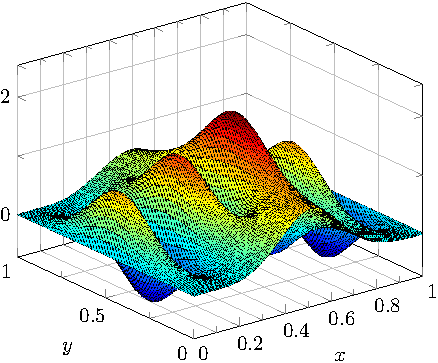
\includegraphics[width=0.7\columnwidth]{figures/Example.pdf}
    	\caption{3D surface obtained from PGFPlots \cite{PFGPlots}.}
    	\label{fig:figure}
    \end{figure}

\section{Tables}
	
        \tabref{tab:table} shows an example table of some astronomical objects. 

        \begin{table}[H]
        	\caption{Astronomical Object Data}
        	\label{tab:table}
        	\begin{tabular}{
        		>{\raggedright\arraybackslash}p{0.25\columnwidth}
        		>{\raggedright\arraybackslash}p{0.29\columnwidth}
        		>{\raggedright\arraybackslash}p{0.31\columnwidth}
        	}
        	\toprule
        	\textbf{Object} & \textbf{Type} & \textbf{Distance (Light Years)} \\
        	\midrule
        	Alpha Centauri & Star system & 4.37 \\
        	Betelgeuse & Red supergiant star & 642.5 \\
        	Andromeda & Spiral galaxy & 2.537 million \\
        	Earth & Planet & 0 \\
        	Sirius & Binary star system & 8.6 \\
        	\bottomrule
        	\end{tabular}
        	\tabletext{Note: The table contains data of some famous celestial objects.}
        \end{table}

        The \inlinecode{\tabletext{}} command is used to add notes to tables easily. 

\section{Document Data}

    \subsection{Front-Matter Footer Block*}

        A new block called \inlinecode{\docinfo{}}, has been added to the bottom right of the first page, acting as a floating element which stays fixed in place. This replaces the corresponding author block previously located above the abstract in earlier versions.

        The \inlinecode{\docinfo{}} block was created to give you greater control over supplementary document data, such as publication dates, licensing information, extended author details, and other front-matter notes. You can fully customize its content to suit your needs.

        Additionally, the new \inlinecode{\corres{}} command serves as a flexible alternative to \inlinecode{\thanks{}}. Since modifying the standard \inlinecode{\thanks{}} command can be complex and its positioning is often rigid, \inlinecode{\corres{}} was introduced to offer a more adaptable solution without sacrificing functionality. 
        
        \begin{note}
            You can use \verb|\corres{}| as many times as needed since it automatically ensures that each entry remains correctly associated. For best results, I recommend using text symbols rather than mathematical ones (e.g., \verb|\textasteriskcentered|, \verb|\textdagger|, etc.). 
        \end{note}

        If \inlinecode{\corres{}} is not used, \inlinecode{\docinfo{}} will automatically adjust its position. The implementation was designed to handle any combination of front-matter elements you might need when starting your document. In this example template, you’ll find a minimal demonstration that combines both to illustrate their interaction.

    \subsection{Headers and Footers*}

        \subsubsection{Headers}

            On all pages except the first, the document title and journal appear in the header. Since twoside layout is enabled, its position alternates depending on whether the page is odd or even.

        \subsubsection{Footers}

            In the first page, six elements display supplementary information for your document:

            \begin{itemize}
                \item \inlinecode{\journalname{}} — Displays the journal name, university, institute, company, or any institutional affiliation.
                \item \inlinecode{\theday{}} — Displays the current date.
                \item \inlinecode{\vol{}} — Specifies the volume number of the publication.
                \item \inlinecode{\no{}} — Specifies the issue number within the volume.
                \item \inlinecode{\journal{}} — Defines the full journal title.
                \item \inlinecode{\thepage} — Shows the current page number and the total count.
            \end{itemize}

             In all cases, you can freely rearrange or customize the order of these elements by modifying the class file to suit your needs. If any of them are not required, simply omit the corresponding command — the remaining elements will automatically adjust their spacing to remain evenly distributed.

\section{Rho Custom Packages}

    \subsection{Rhobabel.sty}
		
		This package have all the commands that automatically translate from English to Spanish when this custom package is defined. 
		
		By default, this document has its content in English. However, at the beginning of the document you will find a recommendation when writing in Spanish. 
		
		You may modify this package if you want to use other language than English or Spanish. This will make easier to translate your document without having to modify the class document.

    \subsection{Rhoenvs.sty}

        This package provides custom environments designed to enhance the visual presentation and structure of your document. Key examples include rhoenv, info, and note.
        
		Their style is defined by \inlinecode{rhoenvstyle} — allowing you to customize their appearance according to your document’s requirements.

		An example using the \inlinecode{rhoenv} environment is shown below.
		
		\begin{rhoenv}[frametitle=Custom Title]
			This is an example of the custom title environment. To add a title type this command \verb|[frametitle=Custom Title]| next to the beginning of this environment (as shown in this example).
		\end{rhoenv}

        The \inlinecode{info} and \inlinecode{note} are environments which have a predefined title and translate their title to Spanish automatically when this language is defined.

\section{Equations}

	\equref{eq:equation} shows the Schrödinger equation as an example. 

    \begin{equation}\label{eq:equation}
        i\hbar \frac{\partial }{\partial t}\Psi(\mathbf{r},t) = \left[\frac{-\hbar^2}{2m}\nabla^2 + V(\mathbf{r},t) \right]\Psi(\mathbf{r},t)
    \end{equation}
	
	The \inlinecode{amssymb} and \inlinecode{amsmath} packages were not required, as \href{https://ctan.org/pkg/stix2-otf/}{STIX2} font incorporates mathematical symbols for writing quality equations.
	
	\begin{note}
		If you would like to change the values that adjust the spacing above and below the equations, change the \verb|\eqskip| value until the preferred spacing is set. The default value is set to 9pt.
	\end{note}

\section{Codes}

	\subsection{Coding with Minted*}
	
		The \inlinecode{minted} package offers customized features for adding codes. In addition, the template is designed to work seamlessly with Fira Code, a monospaced font specially crafted for programming environments.

        If your are using a desktop app as \href{https://www.texstudio.org/}{TeXstudio}, try these steps to make this package work on Windows:
		
		\begin{enumerate}
			\item Install Python — A stable version (e.g., v.3.11)
			\item Open the terminal and type \inlinecode{pip install Pygments}.
			\item Update if a newer version is available.
			\item Go to TeXStudio settings and change the default compiler to \inlinecode{pdflatex --shell-escape -interaction=nonstopmode \%.tex}.
			\item Compile and wait for the result.
		\end{enumerate}
        
		\vspace*{-9pt}
        
		\begin{rhoenv}[frametitle=Caution]
			Ensure that \textbf{pygments} is properly installed and added to your system’s PATH. Otherwise, you may encounter compilation errors. Additionally, enable shell escape when compiling, as it is required for minted to process and highlight code.
		\end{rhoenv}
		
		In \href{https://es.overleaf.com/}{Overleaf}, this package is easier to use since it does not require any additional installations or modifications — just add the code as shown in the example. \coderef{lst:example} shows a Python example.
		
		\begin{code}
			\inputminted{python}{example.py}
            \caption{Python code example with minted.}
			\label{lst:example}
		\end{code}
		
		You can customize its design changing \inlinecode{\usemintedstyle} command. The different styles offered by the \href{https://ctan.org/pkg/minted}{minted package} can be preview through this link — \url{https://pygments.org/styles/}.

    \subsection{Coding with Listings}
	
		Since \inlinecode{minted} requires additional installations and can be complex in some desktop \TeX\ editors, you can use the \inlinecode{listings} package instead, which provides a simpler way to include code.
		
		\begin{code}
			\lstinputlisting[language=python]{example.py}
			\label{lst:example2}
            \caption{Python code example with listings.}
		\end{code}
		
		While \inlinecode{listings} is a simpler and widely supported package for code formatting, \inlinecode{minted} offers a more modern and powerful approach. It leverages the Pygments syntax highlighter to deliver superior coloring, language support, and styling options. One of its key advantages is the ability to easily switch between built-in color styles.
		
		In contrast, \inlinecode{listings} requires manual setup for colors, fonts, and formatting rules.
		For users who prefer fine-tuned customization, the styling options for \inlinecode{listings} are organized in \inlinecode{rho.cls} file and can be modified at any time to suit individual preferences.

	\subsection{Inline Code*}
	
		As shown in this template, inline code has a custom style for improved visual appeal. To use it, simply add \inlinecode{\inlinecode{}} command and place your code inside the braces.

\section*{Numberless section}
\addcontentsline{toc}{section}{Numberless section}

    Declaring a numberless section automatically inserts a square symbol before the title. This unique feature is specific to first-level sections within this class.
    
    As this symbol also affects the table of contents and references titles, users who prefer to disable it may edit the section styling parameters in \inlinecode{rho.cls}.

\section{Bibliography}
		
	Bibliography management is handled by \inlinecode{biblatex}, with the default citation and reference style set to IEEE. The \inlinecode{citestyle=numeric-comp} option is enabled, allowing multiple citations to be grouped within a single bracket (e.g., \cite{davis2023signalflow,bell2022codefont}). The citation format can be customized directly in \inlinecode{rho.cls} to suit any preferred style.

\section*{FAQ}
\addcontentsline{toc}{section}{FAQ}

    \subsection*{How do I manage my references?}
    \addcontentsline{toc}{subsection}{How do I manage my references?}
        
        To manage your references, I recommend using the tool \href{https://www.scribbr.es/citar/generador/folders/73QOXYsCwMRu4ifQaN65mx/lists/msTfx7GJjIAOUkufbISnA/}{scribbr}. You can simply enter the URL or create your own citation, and then export it to \LaTeX{} using the options in the three-dot menu.
            
        The generated citation can be copied and pasted into \inlinecode{rho.bib}, the file designated for bibliography management. You may rename this file, but if you do, remember to update the \inlinecode{\addbibresource} command in \inlinecode{rho.cls} under the biblatex section.
    
        \begin{note}
            Some platforms, such as Google Scholar or scientific journals, provide citations directly in BibTeX format. Therefore, check if there is a ``how to cite this document'' section to streamline the citation process even further.
        \end{note}

        If you have any further questions, you can refer to the following page — \href{https://es.overleaf.com/learn/latex/Bibliography_management_with_biblatex}{Bibliography management with biblatex}.
        
    \subsection*{What should I do with the example files?}
    \addcontentsline{toc}{subsection}{What should I do with the example files?}

        The template includes sample content — such as an example figure, bibliography entries, and the \inlinecode{example.py} script — to demonstrate how the layout and features work. Once you start customizing the document for your own use, feel free to delete all example files and entries you don’t need.

    \subsection*{How do I place equations easily?}
    \addcontentsline{toc}{subsection}{How do I place equations easily?}

        For equations, we have two options: inline or on its own line. For inline equations, simply place a dollar sign (\$) at the beginning and end of the equation. However, if you want the equation to be displayed on its own line, you need to use the equation environment.
        
        If you find it challenging to write formulas directly in \LaTeX, you can use text editors like Word. In the equations menu, you can select \LaTeX\ in the conversion section and copy and paste the equation you wrote into one of these two environments.

    \subsection*{How do I change the paper size?}
    \addcontentsline{toc}{subsection}{How do I change the paper size?}

        By default, this class was adapted for a4paper and test it with letterpaper. The following paper sizes are available in \LaTeX:

        \begin{itemize}
            \item letterpaper (11 $\times$ 8.5 in)
            \item legalpaper (14 $\times$ 8.5 in)
            \item executivepaper (10.5 $\times$ 7.25 in)
            \item a4paper (21 $\times$ 29.7 cm)
            \item a5paper (21 $\times$ 14.8 cm)
            \item b5paper (25 $\times$ 17.6 cm)
       \end{itemize}

\section*{Contact me}
\addcontentsline{toc}{section}{Contact me}
    
    Have questions, suggestions, or an idea for a new feature? Found a bug or working on a project you’d like to invite me to?  
    
    Feel free to reach out — I’d be happy to help, collaborate, or fix the issue.  Your feedback helps me improve my templates!

    \AtBeginEnvironment{tabular}{\normalsize\sffamily\selectfont}
    \begin{center}
        \setlength{\tabcolsep}{3pt}
        \begin{tabular}{cl}
            \faEnvelope & \href{mailto:memo.notess1@gmail.com}{memo.notess1@gmail.com} \\
            \faGlobe{} & \href{https://memonotess1.wixsite.com/memonotess}{memonotess.com} \\
            \faInstagram{} & \href{https://www.instagram.com/memo.notess/}{@memo.notess}
        \end{tabular}
    \end{center}

\section*{Github Repository}
\addcontentsline{toc}{section}{Github Repository}

    Visit the repository to access the source code, track ongoing development, report issues, and stay up to date with the latest changes.

    \begin{center}
        \setlength{\tabcolsep}{3pt}
        \begin{tabular}{cl}
             \faGithub &  \url{https://github.com/MemoJimenez/Rho-class}\\
        \end{tabular}
    \end{center}

\section*{Supporting}
\addcontentsline{toc}{section}{Supporting}

    Enjoyed this document class? Check out tau-class, my very first \LaTeX{} template.

    \begin{center}
        \setlength{\tabcolsep}{3pt}
        \begin{tabular}{cl}
             \faLink &  \href{https://es.overleaf.com/latex/templates/tau-class-lab-report-template/chhshmhxstsq}{https://es.overleaf.com/latex/templates/tau-class}\\
        \end{tabular}
    \end{center}
    
    \subsection*{Any contributions are welcome!}
    \addcontentsline{toc}{subsection}{Any contributions are welcome!}
    
        Coffee keeps me awake and helps me create better \LaTeX\ templates. If you wish to support my work, you can do so through PayPal: 

        \begin{center}
            \setlength{\tabcolsep}{3pt}
            \begin{tabular}{cl}
                 \faPaypal & \textbf{\url{https://www.paypal.me/GuillermoJimeenez}}\\
            \end{tabular}
            \vskip9pt
            Enjoy writing with rho-class!
        \end{center}

%----------------------------------------------------------

\printbibliography

%----------------------------------------------------------

\end{document}